%%%%%%%%%%%%%%%%%%%%%%%%%%%%%%%%%%%%%%%%%%%%%%%%%%%%%%%%%%%%%%%%%%%%%%%%%%%%%%%%
% Uncertainties and Results:
%%%%%%%%%%%%%%%%%%%%%%%%%%%%%%%%%%%%%%%%%%%%%%%%%%%%%%%%%%%%%%%%%%%%%%%%%%%%%%%%
\chapter{Statistical Analysis, Uncertainties and Results}
\label{statAnalysis_uncerts_results}
%%%%%%%%%%%%%%%%%%%%%%%%%%%%%%%%%%%%%%%%%%%%%%%%%%%%%%%%%%%%%%%%%%%%%%%%%%%%%%%%
The results and their uncertainties obtained in this search are presented here.  Evidence in 
support of a \WR and \nul signal was sought in finite sized windows of $\Mlljj$, whose sizes 
were chosen to minimize the upper bound \WR cross section limit in the absence of a signal.  
Uncertainties that affected the background and signal estimates were measured in each $\Mlljj$ 
window.  The main uncertainties that affected the background estimate arose from limited event 
statistics in $e\mu$ data, and discrepancies between data and simulations in \DY-rich control 
regions.  The main uncertainties that affected the signal estimate came from luminosity and 
pileup measurements in data.  Additional sources of uncertainty existed and were measured, 
but had a smaller cumulative impact on the results.  Following uncertainty estimation, the 
results were obtained by comparing data, expected SM backgrounds and hypothetical 
\WR and \nul signals using the $\Mlljj$ distribution, and limits on the \WR cross section, 
$\mWR$ and $\mnul$ masses derived from data and expected backgrounds.

%%%%%%%%%%%%%%%%%%%%%%%%%%%%%%%%%%%%%%%%%%%%%%%%%%%%%%%%%%%%%%%%%%%%%%%%%%%%%%%%
% Statistical Analysis and Uncertainties 
%%%%%%%%%%%%%%%%%%%%%%%%%%%%%%%%%%%%%%%%%%%%%%%%%%%%%%%%%%%%%%%%%%%%%%%%%%%%%%%%
\section{Statistical Analysis and Uncertainties}
\label{sec:massWindows_uncertainties}
%%%%%%%%%%%%%%%%%%%%%%%%%%%%%%%%%%%%%%%%%%%%%%%%%%%%%%%%%%%%%%%%%%%%%%%%%%%%%%%%
The $\Mlljj$ signature of \WR and \nul signals considered in this search were characterized 
by distributions that peaked at \mWR, and had tails that extended several hundred $\GeV$ 
below and above the peak.  The only other assumption made regarding the shape of signals in 
$\Mlljj$ was that the tails grew larger as \mWR increased, as shown in Figure \ref{fig:fig:signalShapesAfterSelection}.  
The.

\begin{figure}[btp]
	\centering
	\subfigure{
		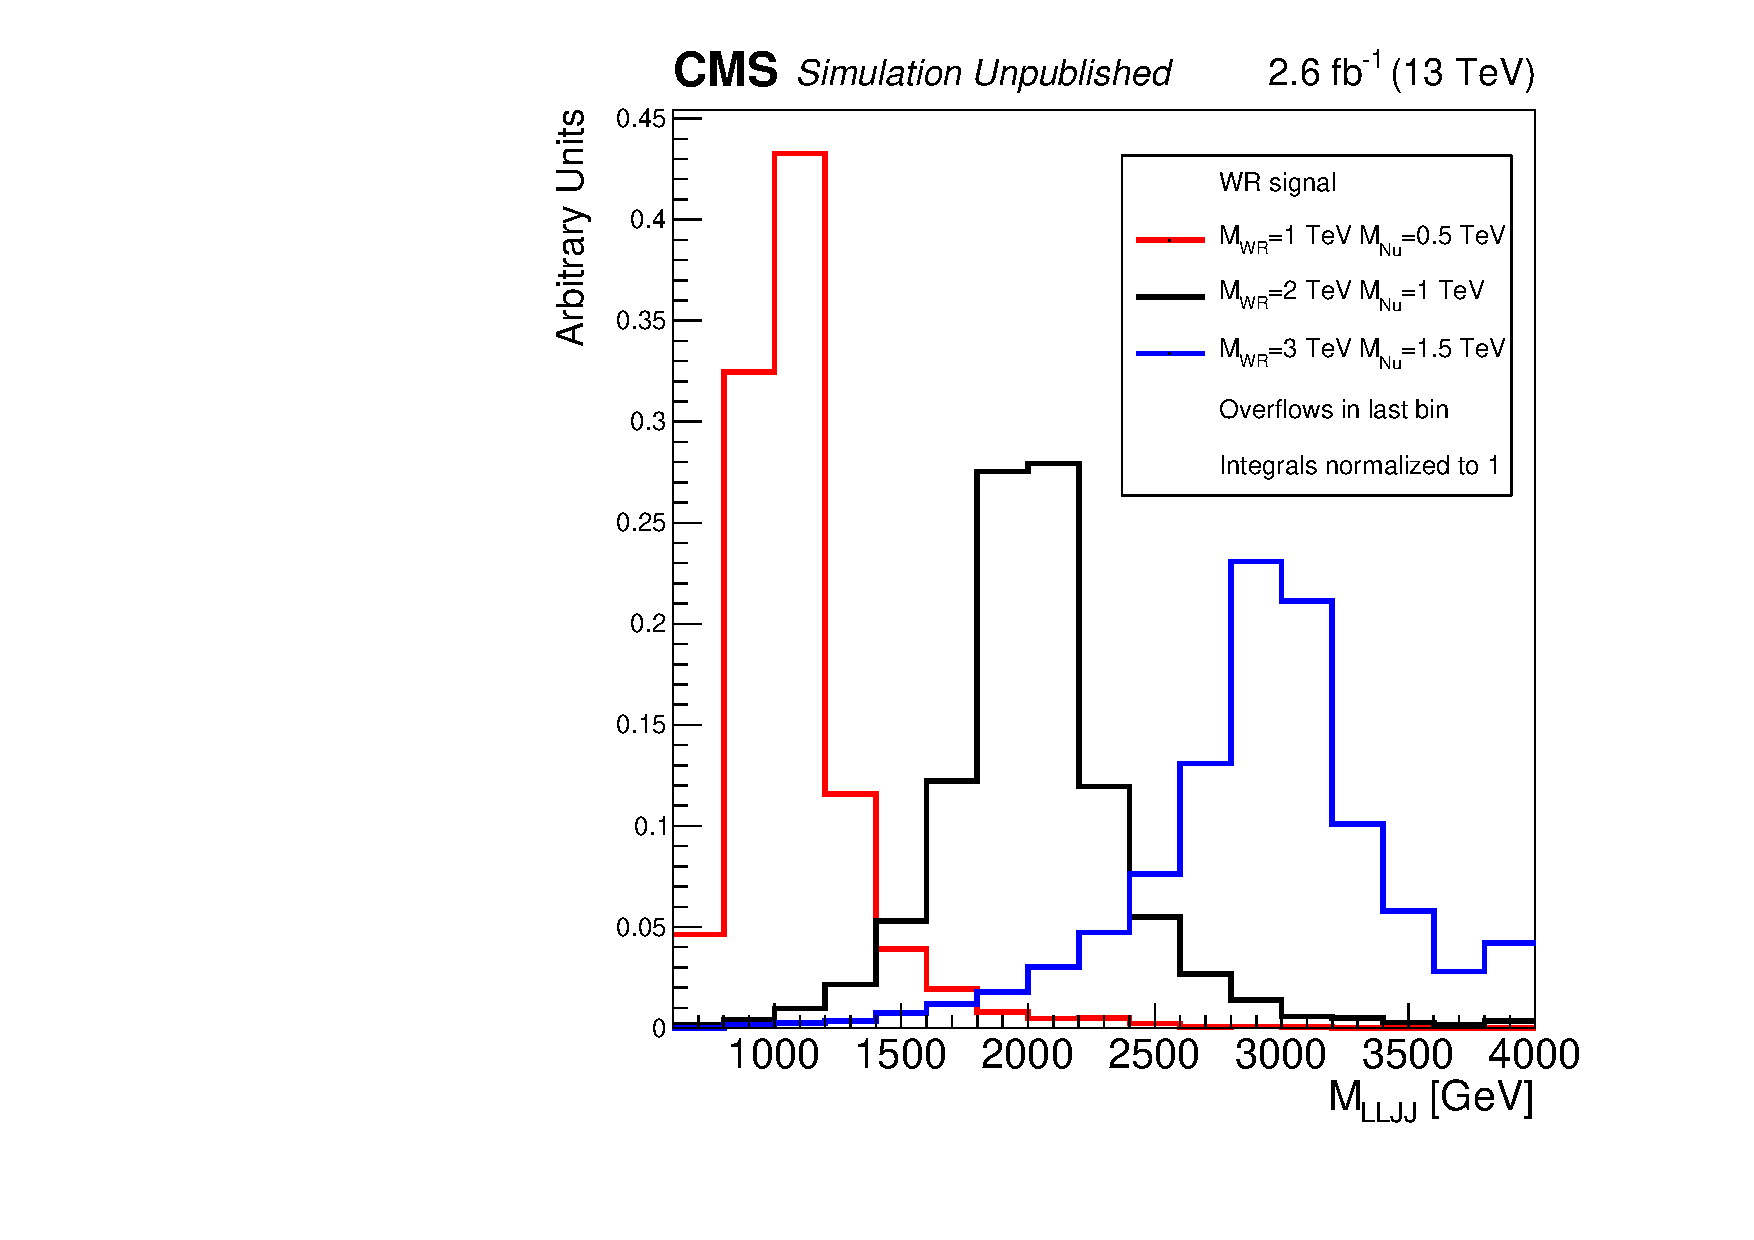
\includegraphics[width=0.45\textwidth]{figures/Mlljj_signalRegionCuts_severalWrSignals_EE.pdf}
	}
	\subfigure{
		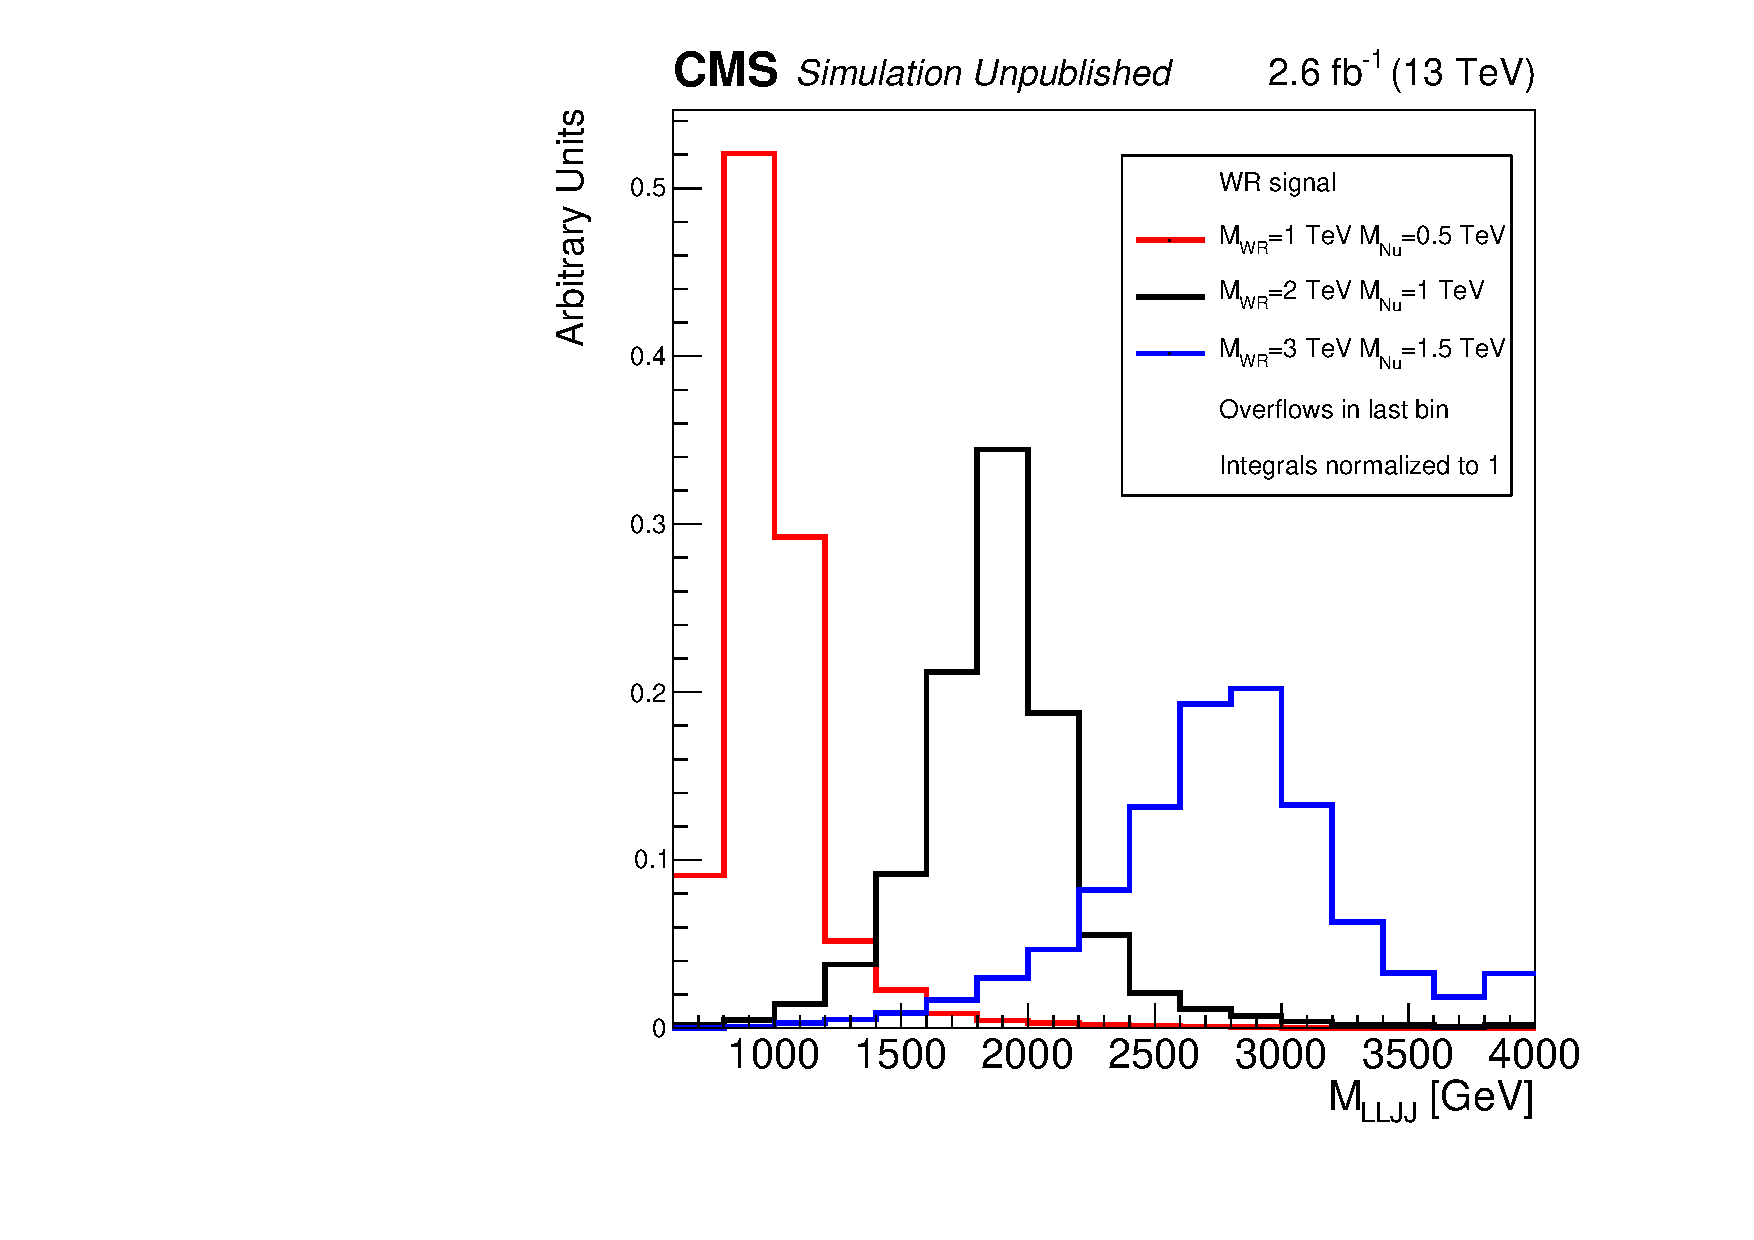
\includegraphics[width=0.45\textwidth]{figures/Mlljj_signalRegionCuts_severalWrSignals_MuMu.pdf}
	}
	\label{fig:signalShapesAfterSelection}
	\caption{$\Mlljj$ distribution after all selections for several \WR signal hypotheses in the $ee$ (left) and $\mu\mu$ (right) 
		channels.  The tails of the distribution grew as \mWR increased.}
\end{figure}


For each \mWR mass hypothesis, a $\Mlljj$ window ($ min < \Mlljj < max$) was defined such 
that the expected upper limit\footnote{The expected limit was calculated by setting the 
number of observed events equal to the number of events expected from SM backgrounds.} on 
the \WR cross section was minimized.  In each window the limit was calculated by counting 
the number of events that fell in the window, without regard to the shape of their distribution, 
using a procedure described later in Chapter \ref{sec:searchResults}.  The windows used 
for each \mWR mass hypothesis, shown in Table \ref{tab:masscuts}, were chosen such that the expected upper 
limit on the \WR cross section was minimized.

\begin{table}[h]
\caption{$\Mlljj$ window ranges that minimized the expected upper limit on the \WR cross section at different \mWR values.}
\label{tab:masscuts}
\centering
\begin{tabular}{|c|r@{ - }l|r@{ - }l|} \hline
\mWR (\GeV) & \multicolumn{4}{c|}{\Mlljj window (\GeV)}  \\\hline
& \multicolumn{2}{c|}{Electrons}  & \multicolumn{2}{c|}{Muons}  \\  \hline
 800  & 700       &  1100       &  700       &  1200      \\  \hline
1000  & 900       &  1300       &  900       &  1400      \\  \hline
1200  & 1100       &  1550       &  1100       &  1650      \\  \hline
1400  & 1250       &  1750       &  1300       &  1850      \\  \hline
1600  & 1450      &  2000       &  1500      &  2100      \\  \hline
1800  & 1600      &  2250       &  1600      &  2300      \\  \hline
2000  & 1850      &  2550       &  1850      &  2600      \\  \hline
2200  & 2000      &  2800       &  2000      &  2850      \\  \hline
2400  & 2150      &  3100       &  2150      &  3100      \\  \hline
2600  & 2250      &  3400       &  2300      &  3400      \\  \hline
2800  & 2350      &  3700       &  2400      &  3700      \\  \hline
3000  & 2500      &  4000       &  2500      &  3950      \\  \hline
3200  & 2550      &  4300       &  2700      &  4250      \\  \hline
3600  & 2700      &  4900       &  2900      &  4850      \\  \hline
3800  & 2750      &  5200       &  2950      &  5150      \\  \hline
4000  & 2800      &  5500       &  3000      &  5450      \\  \hline
4200  & 2800      &  5750       &  3100      &  5750      \\  \hline
4400  & 2850      &  6050       &  3150      &  6100      \\  \hline
4600  & 2850      &  6300       &  3150      &  6400      \\  \hline
4800  & 2850      &  6600       &  3200      &  6700      \\  \hline
5000  & 2900      &  6850       &  3200      &  7000      \\  \hline
5200  & 2900      &  7050       &  3200      &  7300      \\  \hline
5600  & 2900      &  7500       &  3200      &  7850      \\  \hline
5800  & 2950      &  7700       &  3200      &  8150      \\  \hline
6000  & 2950      &  7900       &  3200      &  8400      \\  \hline
\end{tabular}
\end{table}




%%%%%%%%%%%%%%%%%%%%%%%%%%%%%%%%%%%%%%%%%%%%%%%%%%%%%%%%%%%%%%%%%%%%%%%%%%%%%%%%
% Results
%%%%%%%%%%%%%%%%%%%%%%%%%%%%%%%%%%%%%%%%%%%%%%%%%%%%%%%%%%%%%%%%%%%%%%%%%%%%%%%%
\section{Results}
\label{sec:searchResults}
%describe how limits are calculated with and without syst uncertainties before showing results
%when explaining limit calculation procedure without syst uncertainties, refer back to 
%Chapter \ref{sec:massWindows_uncertainties}

%%%%%%%%%%%%%%%%%%%%%%%%%%%%%%%%%%%%%%%%%%%%%%%%%%%%%%%%%%%%%%%%%%%%%%%%%%%%%
